\documentclass{article}

\usepackage{corl_2023} % Use this for the initial submission.
%\usepackage[final]{corl_2023} % Uncomment for the camera-ready ``final'' version.
%\usepackage[preprint]{corl_2023} % Uncomment for pre-prints (e.g., arxiv); This is like ``final'', but will remove the CORL footnote.

% ### custom packages start ###
% math
\usepackage{amsmath,amsfonts,amssymb,amsthm}
\usepackage{mathtools}
\usepackage{commath}
\DeclareMathOperator*{\argmax}{arg\,max}
\DeclareMathOperator*{\argmin}{arg\,min}

% tables
\usepackage{array}
\usepackage{booktabs}
\usepackage{multirow}

% figures
\usepackage{subcaption}
\usepackage{wrapfig}

% algorithms
\usepackage{algorithm}
\usepackage{algpseudocode}
\newcommand{\minuseq}{\mathrel{-}=}

% colors
\usepackage{color}  % CoRL uses color insted of xcolor.
\definecolor{purple}{rgb}{0.5,0.0,0.5}
\definecolor{olive}{rgb}{0.5,0.5,0.0}
\newcommand{\ob}[1]{\textcolor{purple}{[\textbf{OB:} #1]}}
\newcommand{\evdp}[1]{\textcolor{blue}{[\textbf{EvdP:} #1]}}
\newcommand{\lsw}[1]{\textcolor{olive}{[\textbf{lsw:} #1]}}
\newcommand{\rob}[1]{\textcolor{green}{[\textbf{rob:} #1]}}
\newcommand{\tk}[1]{\textcolor{magenta}{[\textbf{TK:} #1]}}
\newcommand{\rst}
[1]{\textcolor{red}
{[\textbf{ST:} #1]}}


% highlight
\usepackage{soul}
\definecolor{lightlightgrey}{rgb}{0.9,0.9,0.9}
\sethlcolor{lightlightgrey}

% notation
\newcommand{\pcx}[1]{\mathrm{pcd}^{(#1)}}
\newcommand{\wxy}[2]{W_{#1 \rightarrow #2}}
\newcommand{\pci}{\pcx{i}}
\newcommand{\pcj}{\pcx{j}}
\newcommand{\pcc}{\pcx{C}}
\newcommand{\wij}{\wxy{i}{j}}
\newcommand{\wci}{\wxy{C}{i}}

% ### custom packages end ###

% \title{SA-Warp: Simple $\mathrm{SE}(3)$ Object Re-arrangement \\via Shape and Action Warping}

% \title{Simple $\mathrm{SE}(3)$ Object Re-arrangement \\via Shape and Action Warping}

% didn't like the title above, but not sure how I feel about this one either...
\title{One-Shot Imitation Learning via Shape Warping}

% The \author macro works with any number of authors. There are two
% commands used to separate the names and addresses of multiple
% authors: \And and \AND.
%
% Using \And between authors leaves it to LaTeX to determine where to
% break the lines. Using \AND forces a line break at that point. So,
% if LaTeX puts 3 of 4 authors names on the first line, and the last
% on the second line, try using \AND instead of \And before the third
% author name.

% NOTE: authors will be visible only in the camera-ready and preprint versions (i.e., when using the option 'final' or 'preprint'). 
% 	For the initial submission the authors will be anonymized.

\author{
  Jane E.~Doe\\
  Department of Electrical Engineering and Computer Sciences\\
  University of California Berkeley 
  United States\\
  \texttt{janedoe@berkeley.edu} \\
}


\begin{document}
\maketitle

%===============================================================================

\begin{abstract}
TODO
\end{abstract}

% Two or three meaningful keywords should be added here
\keywords{TODO} 

%===============================================================================

\begin{figure}[h]
    \centering
    \includegraphics[width=\textwidth]{figures/figure_9.pdf}
    \caption{Examples of real-world generalization capabilities of SA-Warp. \ob{TODO: Reduce visual clutter, maybe masking or blurring.}}
    \label{fig:intro}
\end{figure}

\section{Introduction}
% OB: I moved the prior version and comments to 'latex/scratch.tex' in this overleaf project.

Robot learning of manipulation policies in the open world -- in situations, and to objects, the robot has not previously encountered -- is a grand challenge in robotics. An important aspect of this problem is our representation of the 3D world. Our paper focuses on a factored representation of the world, where we first find all objects of interest and then represent the 3D shape of each object independently. Our representation should generalize to unfamiliar objects in unfamiliar environments. For example, a robot should be able to enter a new kitchen and place a mug of a new shape on a hook (Figure \ref{fig:intro}). Additionally, we wish the robot to generalize to objects placed in novel positions and orientations. E.g. the robot should be able to pick a mug laying sideways on a floor even if it has previously only seen mugs standing on a countertop. We call this property $\mathrm{SE}(3)$-equivariance.

Classical robotics approaches represent objects using explicit 3D geometries. \citet{miller03automatic,tenorth13decomposing} decompose complex objects into primitive shapes to plan for grasps and \citet{klank09realtime,beetz11robotic} rely on having CAD models of all objects in the world. The generalization ability of these approaches is limited, as these hand-crafted 3D representations cannot be accurately fit to any new object the robot encounters. To address this limitation, recent approaches use implicitly learned 3D descriptors. \citet{mescheder19occupancy,park19deepsdf} represent the 3D surface of an object as a decision boundary of a binary classifier neural network. Each 3D point nearby the surface of the object can then be described using the activations of the neural network \cite{simeonov22neural}. \citet{pan22taxpose} use neural point cloud embeddings \cite{qi17pointneta} and cross-attention \cite{vaswani17attention} to learn point cloud representations that are comparable between object instances.

Implicit 3D descriptors have led to impressive results in few-shot 3D manipulation. Neural Descriptor Fields (NDFs) \cite{simeonov22neural,simeonov22se} and TAX-Pose \cite{pan22taxpose} learn object re-arrangement policies, e.g. hanging a mug on a hook, from 5 - 10 demonstrations. NDFs use 3D descriptors to match task-relevant object parts between different instances of objects. For example, they align the handles of differently shaped mugs in order to successfully hang them. Alternatively, Tax-Pose computes the cross-attention between the child (mug) and the parent (hook) objects in order to find which parts of the two objects should be nearby each other in the target configuration (mug on tree). The direct comparison between the child and the parent objects can lead to higher accuracy than in NDFs. But, both NDFs and Tax-Pose have two important limitations: (1) a large collection of 3D meshes is required for pre-training (200 objects per category from ShapeNet \cite{chang15shapenet}) and (2) without explicit 3D geometries, it is difficult to perform collision checking and motion planning on a physical robot.

Our paper focuses on an alternative and highly sample-efficient explicit 3D geometry representation method based on \textit{shape warping} \citep{jakel12learning,brandi14generalizing,lee15learning,schulman16learning,rodriguez18transferring,rodriguez18transferringa,thompson21shapebased}. The core idea is to pick a canonical example of an object class, and warp its point cloud (or mesh) to conform to the observations of novel object instances \cite{myronenko10pointset,hillenbrand12transferring,benamor12generalization}. The immediate benefit is that we do not have to represent the shape of an object, but only the \textit{displacement} of points as they are warped between different object instances (belonging to the same object class). We base our method on prior work by \citet{rodriguez18transferring,thompson21shapebased}, who propose to use gradient-descent-based inference to enable shape warping to partial point clouds.
% \tk{We base our method on ... [or mention this connection later in the method section, might not be needed here]} 

We propose \textbf{Shape and Action Warping (SA-Warp)}, a general method for one-shot learning of robotic manipulation policies. First, we propose a new algorithm for the joint inference of object shape, scale, translation and orientation based on its partial point cloud. The algorithm is based on canonical object warping with a low-dimensional latent space of shapes \cite{rodriguez18transferring,thompson21shapebased} and returns a warped 3D mesh. Second, we propose a method for the warping of robot actions. We focus on actions where two objects come into contact: e.g., grasping, relative object placement (e.g. mug on tree) and trajectory cloning with contacts (e.g. painting with a brush on a canvas). Our method finds the \textit{interaction points} between pairs of objects, anchors them to their canonical counterparts, and warps them to conform to objects of novel shapes. We developed SA-Warp specifically for on-robot behavior cloning, and we extensively test it in real-world robot experiments.

\section{Related Work}

\subsection{Imitation Learning from Few Demonstrations} 

We build on a body of robotics work aimed at learning generalizable manipulation policies from few demonstrations. A seminal idea in the literature is a key-point-based representation of objects. \citet{manuelli19kpam} manually create a dataset of semantically meaningful key-points, such as the rim and the handle of a mug, and train a classifier to detect key-points on novel object instances. A task is defined as a time series of key-point positions. Then, a trajectory for a previously unseen object can be computed by matching the key-points on the novel object to the key-point positions seen in a demonstration. In comparison, our method does not require a manual labeling of key-points -- we use the inferred geometry of objects to automatically extract interaction points. \citet{gao21kpam,gao21kpamsc} further extend the key-point framework with feedback control and collision checking. ... also ... \cite{1910,vecerik20s3k,manuelli20keypoints,turpin21gift}.

A related idea is the learning of descriptors attached to arbitrary 2D or 3D key-points. \citet{florence18dense} use self-supervised learning to learn dense descriptors from images. These descriptors can be used to compute similarities of arbitrary key-points between different instances and poses of objects. \citet{chen22neural} compute descriptors of an arbitrary 3D coordinate, called Neural Descriptor Fields, using an implicit shape representation neural network conditioned on a point cloud \cite{mescheder19occupancy}. By attaching a pose of an object to a set of descriptors, they can match e.g.~the pose of a handle of a mug across different mug instances and poses. The method is used re-arrange objects with a variable initial pose and a fixed goal. \citet{simeonov22se} represent pairs of objects using Neural Descriptor Fields to enable generalization across goal poses. \citet{chun23local} further leverage the locality bias of Neural Descriptor Fields to generalize demonstrations across object classes.

Some works rely on CAD model matching to reproduce grasps or manipulation trajectories  \cite{klank09realtime,brook11collaborative,beetz11robotic,jakel12learning}. ... also shape primitives \cite{miller03automatic} ... But, it can be difficult to generalize these methods to novel instances of objects. Recently, \citet{wen22you} tackled category-level manipulation by re-mapping key poses of objects across instances. \citet{pan22taxpose} make predictions about the desired pose of a child object related to a parent object (e.g. hanging a mug on a mug-tree) using cross-attention [] between the pair of point clouds.


\subsection{Shape Warping and Manipulation}

Prior works explored the idea of learning a generative model of point clouds through non-rigid point cloud registration \cite{rodriguez18transferring,rodriguez18transferringa,klamt18supervised,thompson21shapebased}. The model is used to grasp objects based on partial point clouds \cite{rodriguez18transferring,rodriguez18transferringa,klamt18supervised} and to parameterize motion primitives \cite{thompson21shapebased}. In contrast, we learn a generative model of meshes, which we use to find interaction points in demonstrations of manipulation tasks, which in turn enable generalization across object instances. In addition, the pose of objects is either assumed to be given \cite{thompson21shapebased} or detected using a neural pose detector \cite{klamt18supervised}. We propose joint shape and pose inference using gradient descent with random restarts. Gradient descent on both the pose and the shape was used in \cite{rodriguez18transferring,rodriguez18transferringa}, but only to correct for minor deviations in pose. ... also \cite{simeonov20long,you21omnihang,menon22viewpoint,lu22online,wen22you,cong23comprehensive} ...

A second related line work is focused on detecting the contacts between a gripper and an object, and then warping the contact points to fit a novel object \cite{li07datadriven,benamor12generalization,hillenbrand12transferring,jakel12learning,stouraitis15functional,rodriguez18learning,pavlichenko19autonomous,tian19transferring} ... and others ... Instead of directly warping the contact points, we first register them on the canonical mesh corresponding to the grasped object class. This way, we can predict grasps based on partial point clouds; we can even grasp a part of the object that is visually occluded. \ob{I could make a figure for this.}

Finally, point cloud warping has been used to manipulate deformable objects \cite{lee15learning,schulman16learning} and to parameterize a pouring skill \cite{brandi14generalizing}.


%-- \cite{rodriguez18transferring,rodriguez18transferringa}: Similar to Skye's method; they learn a latent space of displacements w.r.t. a canonical point cloud using PCA. During inference, they use gradient descent to solve for both shape and pose. But, they do not tackle the problem of local minima and hence require the shapes to be already almost in alignment. I could give the example of a handle of a mug getting hidden because of local minima and how we solve that. They then use the latent space to somehow warp the grasp actions of a humanoid hand.

\section{Background: Shape Warping by CPD and Gradient Descent}
\label{sec:background}

\begin{figure}
    \centering
    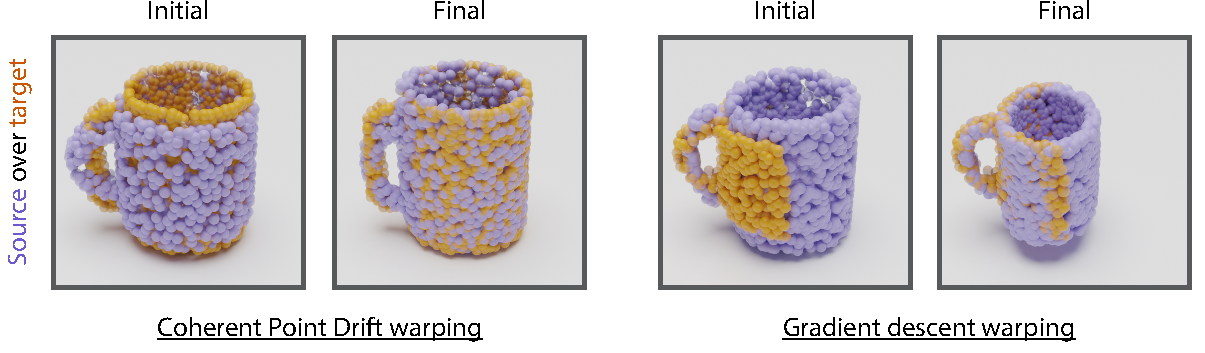
\includegraphics[width=\textwidth]{figures/warping.pdf}
    \caption{Example of warping using CPD and gradient descent with a latent space of warps of a canonical mug. Gradient descent warping works with partial point clouds.}
    \label{fig:warping}
\end{figure}

Shape warping aims to find the correspondence between the shape of two objects by altering one shape to fit the other (Figure \ref{fig:warping}). Usually, the first step is to turn both objects into point clouds. This can be accomplished by sampling the surface or the volume of the object, or directly using the vertices that make up the mesh of the object. Given a pair of point clouds to be matched, shape warping draws on the literature of non-rigid point cloud registration \cite{huang21comprehensive}. Next, we outline the Coherent Point Drift algorithm \cite{manuelli20keypoints}, a common method for aligning a pair of point clouds. We also introduce the necessary notation we will use throughout the paper.
%\rob{This section is not nearly as clear as it should be. You should describe CPD as if you were teaching the method to someone who is new to it. The section is a little short; but most importantly, you introduce new notation when it seems unnecessary and present ideas in a way that makes it hard to follow.}

Denote a pair of point clouds $\pci$ and $\pcj$. We want to compute a matrix of displacements $\wij$ that minimizes some distance function between $\pci + \wij$ and $\pcj$, such as the one-sided Chamfer distance:
\begin{align}
    d\left( \pci + \wij, \pcj \right) = \frac{1}{|\pcj|} \sum_{k=1}^{|\pcj|} \min_{l=1}^{|\pci|} \norm{ \pci_l - \pcj_k }_2.
\end{align}
Note that the two point clouds can have a different number of points. In general, $\wij$ can re-arrange $\pci$ in an arbitrary way, leading to a mapping that is not useful. The Coherent Point Drift (CPD) algorithm regularizes $\wij$ so that nearby points in $\pci$ are displaced similarly. CPD formulates the problem as a fitting of a Gaussian Mixture Model (GMM), where $\pci$ is a set of components and $\pcj$ is the data. It uses expectation maximization to optimize the objective function
\begin{align}
    J(\wij) = - \sum_{k=1}^{|\pcj|} \log \sum_{l=1}^{|\pci|} \exp \left( \frac{1}{2 \sigma^2} \norm{\pcj_k - (\pci + \wij)_l} \right) + \frac{\alpha}{2} \phi(\wij).
\end{align}
The regularizer $\phi$ penalizes high frequencies in $\wij$, so that the displacements applied to $\pci$ do not oscillate among nearby points.

\citet{rodriguez18transferring} observed that we can treat each displacement matrix $\wij$ as a data point in order to learn a generative model of object shapes. Given a canonical object $\pcc$ and a set of warps $\{ \wci \}_{i=1}^K$, each matrix $\wci$ is flattened and treated as a feature vector. Then, we fit a PCA projection matrix $W \in \mathbb{R}^{|\pcc|{\times}D}$ to the data, which allows us to represent each shape by a low-dimensional latent vector $v$:
\begin{align}
    \pcx{v} = \pcc + W v.
\end{align}
Given a new point cloud $\pci$, we infer its shape by solving the following optimization problem by gradient descent:
\begin{align}
    v^* = \argmin_{v \in \mathbb{R}^D} d(\pcc + W v, \pci).
\end{align}
Finally, the term $Wv$ can be replaced by a more expressive model, e.g. an auto-encoder \cite{thompson21shapebased} or possibly a diffusion model \cite{nichol22pointe}. We use PCA for simplicity.

%That is, the matrices are flattened and then compressed by Principal Component Analysis \cite{rodriguez18transferring,rodriguez18transferringa,thompson21shapebased} or by an auto-encoder \cite{thompson21shapebased}. As a result, a low-dimensional feature vector $v$ produces a warped object: $\pcx{v} = \pcc + f(v)$. Here, $f$, which can be a PCA or an auto-encoder, maps a $D$-dimensional vector to the space of $N{\times}3$ canonical point displacements. As we describe in Section \ref{sec:methods:scene}, we can optimize $v$ using gradient descent to recover a full mesh (as well as its pose) from a partial point cloud (Figure \ref{fig:warping}, right).

%Object warping alters the mesh of an object, so that it approximately matches the shape of a different object, usually from the same class. Most object warping approaches turn object meshes into point clouds, which can be warped using techniques from non-rigid Point Set Registration \cite{zhu19review}. In particular, the Coherent Point Drift (CPD) algorithm \cite{myronenko10pointset} translates each point in the source point cloud independently, but regularizes the movement of points to be coherent in local regions using frequency-basis regularization. For example, it can warp a small mug onto a larger mug (Figure \ref{fig:warping}, left) without pulling it inside out, which would be incoherent.

%Formally, given two point clouds $\mathrm{pcd}_i$ and $\mathrm{pcd}_j$, CPD predicts a matrix of translations $W_{i \rightarrow j}$, such that $\mathrm{pcd}_i + W_{i \rightarrow j} \approx \mathrm{pcd}_j$. The shape of $W_{i \rightarrow j}$ is $N{\times}3$, where $N$ is the number of points in $\mathrm{pcd}_i$. Note that each point cloud can have a different number of points; the difference between the point clouds is computed using a matching function, such as the Chamfer distance.

%Prior object warping works have further learned a low dimensional latent space of warps. Given a canonical object $\mathrm{pcd}_C$ and a set of warps $\{ W_{C \rightarrow i} \}_{i=1}^K$, each matrix $W_{C \rightarrow i}$ is treated as a feature vector. That is, the matrices are flattened and then compressed by Principal Component Analysis \cite{rodriguez18transferring,rodriguez18transferringa,thompson21shapebased} or by an auto-encoder \cite{thompson21shapebased}. As a result, a low-dimensional feature vector $v$ produces a warped object: $\mathrm{pcd'} = \mathrm{pcd}_C + f(v)$. Here, $f$ maps a $D$-dimensional vector to the space of $N{\times}3$ canonical point displacements. As we describe in the Methods section \tk{Link to section}, we can optimize $v$ using gradient descent to recover a full mesh (as well as its pose) from a partial point cloud (Figure \ref{fig:warping}, right).

%\section{Problem Statement: $\mathrm{SE(3)}$ Object Re-arrangement}
%\rob{Sorry to be obstinate, but I don't think your method is specific to pick-place. It seems like the key objective here is to warp the relative pose between two objects in order to accommodate in-class shape variation. Those two objects could be the gripper and object (grasping) or the relative pose between two objects (placing). This vision of the problem should inform the title of the paper. I would update this whole section and update fig 3 to reflect this.} \ob{Yes, I decided to also include an experiment with trajectory cloning, so I'll change this section.}
%We formulate the object re-arrangement problem as a problem of predicting a pair of 3D homogeneous transforms $(T_\mathrm{pick}, T_\mathrm{rel})$ given an initial segmented point cloud of the scene. The transform $T_\mathrm{pick}$ defines the pose of the robot's gripper that results in a successful pick. Moreover, the way the robot is holding the object should be compatible with the task it is to accomplish. E.g. a mug should be held by the rim so that it can be placed on a mug tree by its handle. The transform $T_\mathrm{rel}$ represents the relative transform between the initial pose of the manipulated object and its target pose. For the mug-tree problem \evdp{mug-tree problem has not been explicitly introduced yet}, we have, informally, $T_{\mathrm{mug-on-tree}} = T_\mathrm{rel} T_{\mathrm{mug-on-ground}}$. Our problem statement is alike \cite{simeonov22neural,simeonov22se}, whereas \cite{pan22taxpose} consider only the prediction of $T_\mathrm{rel}$. Our work as well as \cite{simeonov22neural,simeonov22se,pan22taxpose} solve tasks using open-loop policies; we discuss an extension of our method to closed-loop manipulation in the Conclusion.

\section{Method: SA-Warp}

\begin{figure}
    \centering
    \includegraphics[width=\textwidth]{figures/method_figure2.pdf}
    \caption{Main method figure. I'll fill it in with real-world images later. \rob{I'm thinking instead of a fig that focuses on warping of relative pose between pair of objects. Maybe visualize mug-on-tree (or bottle in box) for diff warped configs, similar to what you do in fig 2 for objects.}}
    \label{fig:method}
\end{figure}

In this section, we propose \textbf{SA-Warp}, a method for behavior cloning of object re-arrangement policies from a single demonstration. \rst{not just SE(3), but also robust to shape. I think it's worth adressing the sample efficiency over number of objects) not just demos, since that's a primary benefit over NDFs and similar} Our method has three main components that make it work on a real-world robot: (1) hybrid mesh and point cloud warping to enable the detection of contact points and collision avoidance during motion planning, (2) joint estimation of object shape and pose in 3D using gradient descent and (3) cloning of contact points and nearby points to enable transfer of pick and place actions across object instances.

\subsection{Latent Space of Meshes}
\label{sec:methods:mesh}

We pre-train SA-Warp with a small number of example objects (ten objects from ShapeNet [] in our experiments) for each object class. We assume to have access to object meshes (same as []) and we sample a point cloud per object using surface sampling. For each class, we select a canonical example $C$ that appears to be the most representative (we describe two possible heuristics in Appendix X). Then, we apply the method of [] described in Section \ref{sec:background} to learn a latent space of object warps. As a result, we can parameterize object shape by a low-dimensional vector $v$:
\begin{align}
    \pcx{v} = \pcc + W v. \tag{3}
\end{align}

For real-world applications, we found it important to have access to the surface of the object shape parameterized by $v$ in addition to its point cloud. If the point cloud of $\pcx{v}$ is dense enough, it is possible to use surface completion methods []. But, we found a simpler approach to work well: we construct the canonical point cloud $\pcc$ as a combination of the actual vertices of object $C$ and points sampled on its surface. By having actual vertices in $\pcx{v}$, we ensure that they can be warped to create a new mesh. We add the surface samples to make the point cloud more uniform -- meshes modeled by people tend to have highly non-uniform distributions of vertices.

Finally, we create a new mesh by extracting the warped vertices from $\pcx{v}$ and keeping the original faces from object $C$. This way of warping vertices can possibly break the mesh (e.g. by intersecting or inverting its faces), but we did not find it to be a problem when performing collision checking for a reasonable range of real-world objects.

\subsection{Fitting a Mesh to an Observed Point Cloud}
\label{sec:methods:scene}

We observe real-world (or simulated) point cloud $\mathrm{scene\_pcd}$ using one to three RGB-D cameras. The cameras are calibrated to the robot's hand and we fuse their outputs into a single point cloud. We detect each object of interest in $\mathrm{scene\_pcd}$ either using clustering and heuristics (Section X) or using pre-trained RGB-based open-vocabulary object detection and instance segmentation models (Section Y).

Using our latent space from Section X, we aim to recover the pose and the complete mesh of each detected object from its point cloud $\mathrm{pcd}$. First, we use the class of the detected object to select a model from Section X -- we have one for each class. We center $\mathrm{pcd}$ and initialize the canonical point cloud with the following parameters:
\begin{align}
    v = \begin{pmatrix} 0 & ... & 0 \end{pmatrix}, s = \begin{pmatrix} 1 & 1 & 1 \end{pmatrix}, t = \begin{pmatrix} 0 & 0 & 0 \end{pmatrix}, r = \begin{pmatrix} 1 & 0 & 0 \\ 0 & 1 & 0 \end{pmatrix}.
\end{align}
The point clouds starts in its canonical form with the latent shape $v$ equal to zero. We set the initial scale $s$ to one, translation $t$ to zero and rotation $r$ to a unit rotation matrix. We use the Gram-Schmidt [] orthogonalization process to turn the six entries in $r$ into a proper 3D rotation matrix $R$. This method has been shown to enable stable learning of rotation matrices [].

We decode the shape and pose parameters into a transformed point cloud
\begin{align}
    \mathrm{dec} = [(\pcc + W v) \odot s] R^T + t,
\end{align}
and define a loss function
\begin{align}
    \mathcal{L} = \underbrace{\frac{1}{|\mathrm{pcd}|} \sum_k^{|\mathrm{pcd}|} \min_l^{|\mathrm{dec}|} \norm{\mathrm{pcd}_k - \mathrm{dec}_l}_2^2}_{\text{(1)}} + \underbrace{\beta \max_l^{|\mathrm{dec}|} \norm{\mathrm{dec}_l}_2^2}_{\text{(2)}}.
\end{align}
The first term in the loss function is a one-sided Chamfer distance between the decoded and the observed point clouds. The second term is a regularizer on the size of the decoded object. Our implementation regularizes the object to fit into the smallest possible ball. Other options are possible, such as directly regularizing $v$ and $s$, regularizing the $L_2$ norm of $\mathrm{dec}$, etc. The main reason for the regularizer is to prevent large predicted meshes in real-world experiments, which might make it impossible to find collision-free motion plans.

We optimize $v, s, t$ and $r$ using the Adam optimizer [] with learning rate $10^{-2}$ for 100 steps. We set $\beta=10^{-2}$. We found the optimization process is prone to getting stuck in local minima; e.g., instead of aligning the handle of the decoded mug with the observed point cloud, the optimizer might change the shape of the decoded mug to hide its handle. Hence, we restart the process with many different random initial rotations and pick the solution with the lowest loss function. Further, we randomly subsample the point clouds at each gradient descent step -- this allows us to run 12 random starting orientations at once on a consumer GPU.

As a result, we get the decoded point cloud $\mathrm{dec}$ (turned into meshes as described in Section X) and its pose represented by $t$ and $R$.

% \tk{The title of this section says "Perception": I would expect some information about how we go from the camera images (which you show in the figures) to the 3D point cloud / mesh representation of individual objects}

% Given an observed, possibly partial, point cloud $\mathrm{pcd}$, our goal is to predict the latent shape $v$ and pose $T$ of the object. We describe this in Algorithm \ref{alg:warp_infer}.

% \rob{Now, we're getting into material that is novel to this paper. If the objective here can be expressed mathematically (e.g. in terms of min and max), that would be nice. Talk about *what* we're doing mathematically. then talk about how we're doing it -- SGD and random restarts.}

% To jointly estimate the pose and shape, we employ a gradient-based optimization approach with multiple random starts. For each random start, we sample a random $3D$ rotation and use fixed initialization for latent shape $v$, translation $t_{\mathrm{local}}$ and scale $s$. We reconstruct a point cloud using $v$, scale it using $s$, and transform it using the rotation and translation. We then calculate the difference between the reconstructed and predicted point cloud and take a gradient descent step with respect to shape, scale and pose using the Adam optimizer []. We also add a regularizer on the size of the reconstructed object controlled by a hyper-parameter $\beta$.

% We use multiple random restarts with different initial rotations because the joint optimization of shape and pose is prone to local minima. For example, if the optimizer cannot align the handle of the mug with the observed point cloud due to an unfavorable random start, it might instead choose to make the handle as small as possible. This behavior is fixed by taking the parameters of the object with the best fit across many random initial rotations.

% \rob{Agree w/ everything Elise says below. Maybe say explicitly what GS does and how BP works there. Cite others who use GS this way.}

% Another problem is the gradient descent with respect to 3D rotations. While previous approaches have directly optimized Euler angles [], which can be tricky \evdp{better to explicitly explain issues e.g. singularities}, we choose a more elegant \evdp{should not call our own approach elegant} approach of directly learning the 3D rotation matrix []. We parameterize the rotation matrix as a $2{\times}3$ matrix $r$ and perform Gram-Schmidt orthogonalization [], which creates a 3D rotation matrix. This process can be backpropagated through to update $r$. \evdp{does having to backpropagate through GS make training expensive? It might be good to add some information about training wall clock time}

\subsection{Action: Warping of Grasps and Placements}
\label{sec:methods:cloning}

\begin{figure}
    \centering
    \begin{subfigure}[b]{0.25\textwidth}
        \centering
        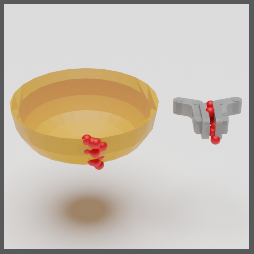
\includegraphics[width=\textwidth]{figures/contact_fig1.pdf}
        \caption{}
    \end{subfigure}
    \hspace{0.05\textwidth}
    \begin{subfigure}[b]{0.25\textwidth}
        \centering
        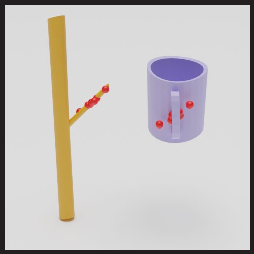
\includegraphics[width=\textwidth]{figures/contact_fig3.pdf}
        \caption{}
    \end{subfigure}
    \hspace{0.05\textwidth}
    \begin{subfigure}[b]{0.25\textwidth}
        \centering
        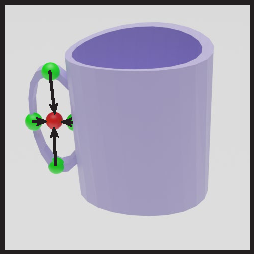
\includegraphics[width=\textwidth]{figures/contact_fig2.pdf}
        \caption{}
    \end{subfigure}
    \caption{(a) Contacts between a gripper and a bowl extracted from a demonstration. (b) Nearby points between a mug and a tree extracted from a demonstration of hanging the mug on the tree. (c) A virtual point (red) representing the branch of the tree intersecting the handle of the mug. The red point is anchored to the mug using k nearest neighbors on the mug (four are shown in green) and moves as the mug warps. All points shown in this visualization are extracted automatically. \ob{TODO: The red point on the mug in (b) are pointing in the wrong way.}}
    \label{fig:contacts}
\end{figure}

\begin{figure}
    \centering
    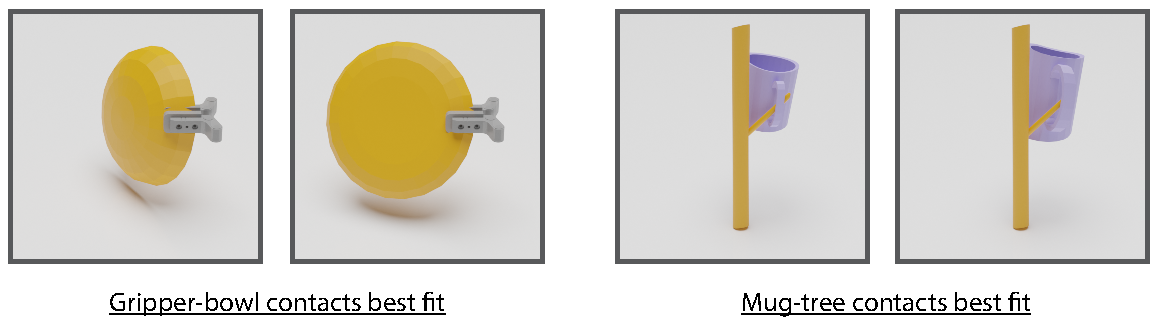
\includegraphics[width=\textwidth]{figures/picks_and_places.pdf}
    \caption{Two solutions for the best fit between the pairs of points on the (left) gripper and child object and (b) the child object and the target object. \evdp{sentence is difficult to parse} We sample the shown meshes from our latent space (Figure \ref{fig:latent}).}
    \label{fig:grasps_and_placements}
\end{figure}

In this section, we describe our approach to clone pick and place actions for different object shapes and poses, given a single demonstration of a task. In general, the demonstration consists of a sequence of $T$ \evdp{is this symbol overloaded? Earlier in the paper capital T (with subscript) referred to transformations} pick and place actions manipulating $M$ objects. Our experiments are restricted to $T=M=2$, but our algorithm is immediately applicable to any sequence, as long as it is told which object to manipulate at which time step. We record the pose of the gripper and the inferred object shape and pose (using Algorithm \ref{alg:warp_infer}):
\begin{align}
    \left(T_{\text{pick/place}}, (v_k, T_k)_{k=1}^M\right)_{t=1}^T
\end{align}

\textbf{Grasp cloning:} To clone a grasp, we register contact points between the gripper and an object. Since we infer the mesh $X$ of the grasped object using Algorithm \ref{alg:warp_infer}, we can sample $B$ contact points between the object mesh and the gripper mesh (Figure \ref{fig:warping}a). For each contact point, we find the nearest neighbor in $X$. We record these indices as $\left< i_1, i_2, ..., i_B \right>$.

When transferring the grasp to a new scene with a different object instance in a different position and orientation, we denote the completed point cloud of the new instance as $Y$. Points $Y_{i_1}, Y_{i_2}, ..., Y_{i_B}$ correspond to the points the gripper touched when picking up the demo object. Since the points have been warped to a new instance, a new grasp could be required. We solve for the best fit between the contact points on $Y$ and the contact points on the gripper (we have pairs of points, where the first point is on the object and the second on the gripper) to get a new grasp pose (Figure \ref{fig:grasps_and_placements}).

\textbf{Placement cloning:} We consider the placement of a child object $X_{\mathrm{child}}$ on a parent object $X_{\mathrm{parent}}$ (e.g. mug on tree, bottle in box) \evdp{what is the definition of a child vs a parent object?}. Given the inferred meshes, we could find the contact points between the child and the parent. However, the two objects might not always touch before the child object is released from the gripper. E.g., when putting an object into a container. Instead, we find nearby points between the child and the parent and anchor them to the child point cloud as \textit{virtual points}.

\rob{Exactly the same comment here as in the grasp section. 1) define the points we're looking for; 2) What properties do these points need to have such that placement is guaranteed to be successful? 3) Does our method deliver? When and when not?}

We find points $p_1, p_2, ..., p_B$ on the parent object that are nearby the child object (Figure \ref{fig:contacts}b). These points are again found based on the inferred meshes of the two objects. For the parent object, we find a nearest neighbor $X_{\mathrm{parent},i_j}$ for each point $p_j$ -- it is the same process as in grasp cloning. For the child object, we anchor each point $p_j$ to its point cloud using its $K$ nearest neighbors $(n_1, n_2, ..., n_k)$. We save the deltas between $p_j$ and its neighbors $\delta = (v_j - n_1, v_j - n_2, ..., v_j - n_k)$ (Figure \ref{fig:contacts}c). Given warped nearest neighbors $n'$, we update $p_j$ as the mean over the deltas to the neighbors:
\begin{align}
    p'_j = \frac{1}{k} \sum_{i=1}^k n'_i + \delta_i.
\end{align}

Using the above method, we can calculate pairs of contact points in a novel scene. We solve for the transformation of the child object so that the contact points are in the best possible alignment with the target object. Finally, we solve for a collision free motion plan that places the child object to the target pose.

\section{Experiments}
\label{sec:exp}

We evaluate both the perception and imitation learning capabilities of SA-Warp. In Section \ref{sec:exp:rearrangement}, we perform three object re-arrangement tasks with previously unseen objects both in simulation and on a physical robot. In Section \ref{sec:exp:trajectory}, we use a painting task to demonstrate that SA-Warp is able to clone manipulation trajectories. In Section \ref{sec:exp:wild}, we show our system is capable of proposing diverse grasps in a cluttered kitchen setting from a single point cloud. We also validate the assumption that we can reliably detect and segment objects; we use a pre-trained vision transformer [metaai segment anything]. Our real-world results amount to about 50 hours of robot data \tk{Used for training / estimation?}.

\subsection{Object Re-arrangement}
\label{sec:exp:rearrangement}

\textbf{Setup:} For our simulated experiment, we use an open-source environment with three tasks: mug on a mug-tree, bowl on a mug and a bottle in a  container \cite{simeonov22se}\footnote{\url{https://github.com/anthonysimeonov/relational_ndf}}. ... our model receives a single demonstration, whereas the baseline has 10; I might report the baseline with different number of demos ... \rst{compare number of objects trained on, too} Given a segmented point cloud of the initial scene, the goal is to predict the pose of the child object relative to the parent object (e.g.~the mug relative to the mug-tree) so that the task constraint is satisfied. The simulation does not test grasp prediction. For our real-world experiment, we perform both grasps and placements based on a single demonstration.

\textbf{Result:} Tables \ref{tab:real_world}, \ref{tab:simulation}, \ref{tab:training}.

\begin{table*}[t!]
    \centering
    \begin{tabular}{lcccccc|cc}
         \toprule
          & \multicolumn{2}{c}{\textbf{Mug on Tree}} & \multicolumn{2}{c}{\textbf{Bowl on Mug}} & \multicolumn{2}{c}{\textbf{Bottle in Container}} & \multicolumn{2}{c}{\textbf{Mean}} \\
         \textbf{Method} & Pick & Pick\&Place & Pick & Pick\&Place & Pick & Pick\&Place & Pick & Pick\&Place \\
         \midrule
         NDF$^1$ & 93.3 & 26.7 & 75.0 & 33.3 & 20.0 & 6.7 & 62.8 & 22.2 \\
         \midrule
         R-NDF & 60.0 & 13.3 & 41.7 & 41.7 & 33.3 & 20.0 & 45.0 & 25.0 \\
         \textbf{SA-Warp} & \textbf{100.0} & \textbf{93.3} & \textbf{83.3} & \textbf{75.0} & \textbf{80.0} & \textbf{73.3} & \textbf{87.8} & \textbf{80.5} \\
         \bottomrule
    \end{tabular}
    \caption{\rob{fill in results!} Success rates of \hl{real-world robot} \evdp{real-world means on a real robot?} pick-and-place experiments with a single demonstration. $^1$The target object (e.g. the mug tree) is in a fixed pose for this experiment.}
    \label{tab:real_world}
\end{table*}

\begin{table}[h]
    \centering
    \begin{tabular}{llcccccc}
        \toprule
          & & \multicolumn{2}{c}{\textbf{Mug on Tree}} & \multicolumn{2}{c}{\textbf{Bowl on Mug}} & \multicolumn{2}{c}{\textbf{Bottle in Container}} \\
         \textbf{Method} & \# Demos & Upright & Arbitrary & Upright & Arbitrary & Upright & Arbitrary \\
         \midrule
         R-NDF & 1 & 60.0 & 51.0 & 69.0 & 68.0 & 19.0 & 8.0 \\
         TAX-Pose & 1 & - & - & - & - & - & - \\
         \textbf{SA-Warp} & 1 & \textbf{86.0} & \textbf{83.0} & \textbf{82.0} & \textbf{84.0} & \textbf{62.0} & \textbf{60.0} \\
         \midrule
         R-NDF & 5 & 88.0 & \textbf{89.0} & 53.0 & 46.0 & 78.0 & 47.0 \\
         TAX-Pose & 5 & - & - & - & - & - & - \\
         \textbf{SA-Warp} & 5 & \textbf{90.0} & 87.0 & \textbf{75.0} & \textbf{77.0} & \textbf{79.0} & \textbf{79.0} \\
         \midrule
         R-NDF & 10 & 71.0 & 70.0 & 69.0 & 60.0 & \textbf{81.0} & 59.0 \\
         TAX-Pose & 10 & - & - & - & - & - & - \\
         \textbf{SA-Warp} & 10 & \textbf{88.0} & \textbf{88.0} & \textbf{83.0} & \textbf{86.0} & 70.0 & \textbf{83.0} \\
         \bottomrule
    \end{tabular}
    \caption{Success rates of predicted target poses of objects in \hl{simulation}. Upright and arbitrary starting object poses.}
    \label{tab:simulation}
\end{table}

\begin{table}[h]
    \centering
    \begin{tabular}{lccc}
        \toprule
         \textbf{Method} & \# Train. Objects & \# Demos. & Labels \\
         \midrule
         NDF & 200 & 5-10 & Yes \\
         R-NDF & 200 & 5-10 & Yes \\
         TAX-Pose & 200 & 5-10 & No \\
         \textbf{SA-Warp} & \textbf{10} & \textbf{1} & \textbf{No} \\
         \bottomrule
    \end{tabular}
    \caption{Required training objects, training demonstrations and additional labeled data across methods.}
    \label{tab:training}
\end{table}



\subsection{Trajectory Cloning}
\label{sec:exp:trajectory}

\textbf{Setup:} We record a single demonstration of a robot painting a particular pattern on a canvas with a brush. We then automatically segment this demonstration into waypoints and record the contact of the brush with the canvas at various waypoints. During testing, the robot uses a different brush and paints on a canvas that is potentially curved. We show that we can make predictions about the object poses that constitute the trajectory regardless of the shape of the brush and the canvas.

\textbf{Result:} \ob{Abhinav}

\subsection{Grasp Prediction in the Wild}
\label{sec:exp:wild}

\textbf{Setup:}
In our project, our primary objective was to predict objects in the wild, so we chose DETIC, an object detection method capable of classifying 20,000+ classes. We concentrated on object detection and 3D semantic segmentation using PointNet. However, we encountered challenges with the PointNet network, which led us to adapt the experiment by performing 2D object detection, specifically for mugs or cups.



We explored various methods for 2D object detection and semantic segmentation in different environments, including YOLO V8 Nano (Class Moderated), OWL ViT Image-Guided Detection, OWL ViT Text-Guided Detection, DETIC Object Detector, and the Segment Anything Model (SAM). Our focus was on the combination of SAM and DETIC, which we applied in home and lab environments to assess their performance and effectiveness.

By employing DETIC for object detection with its vast range of classes, we aimed to improve the accuracy of the pipeline. We then used the output bounding boxes from DETIC as prompts for the SAM model, allowing us to achieve better segmentation results. This combination not only enhanced the overall accuracy and effectiveness of the pipeline but also highlighted the adaptability of the SAM model in various scenarios.

Despite some limitations, our project provided valuable insights into the challenges of object detection and 3D semantic segmentation, emphasizing the importance of a more appropriate dataset and addressing the limitations of the PointNet network. Our efforts in combining DETIC and SAM demonstrated the potential of such an approach for future research in the field.
\ob{Kishore -- RGBD to segmented point clouds to grasp candidates}

% \begin{figure*}[]
%     \centering
%     \begin{subfigure}{(\linewidth - 0.1\linewidth)/6}
%         \centering
%         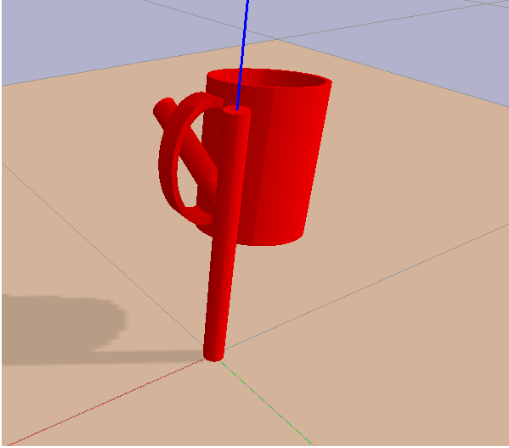
\includegraphics[width=\linewidth]{figures/virtual/1.png}
%         \caption{}
%     \end{subfigure}
%     \begin{subfigure}{(\linewidth - 0.1\linewidth)/6}
%         \centering
%         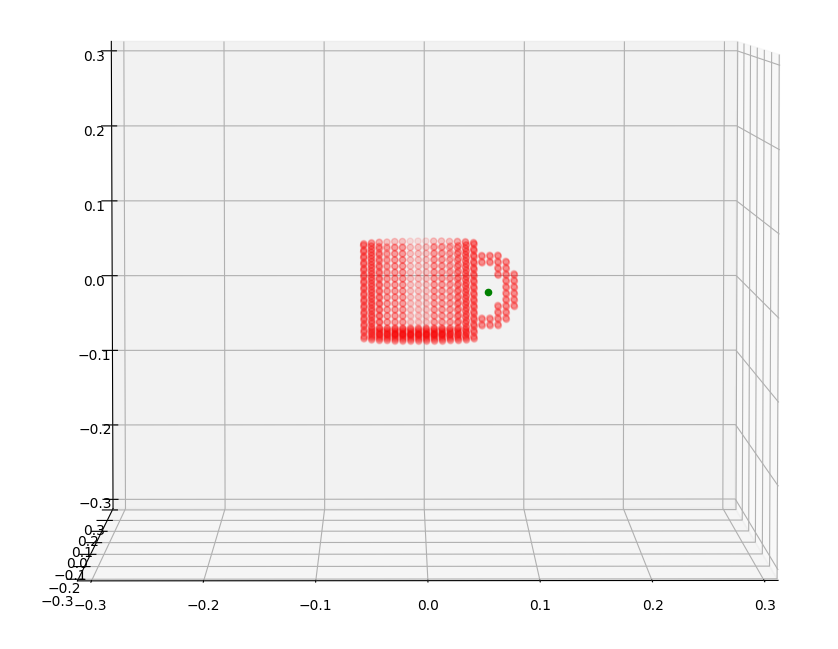
\includegraphics[width=\linewidth]{figures/virtual/2.png}
%         \caption{}
%     \end{subfigure}
%     \begin{subfigure}{(\linewidth - 0.1\linewidth)/6}
%         \centering
%         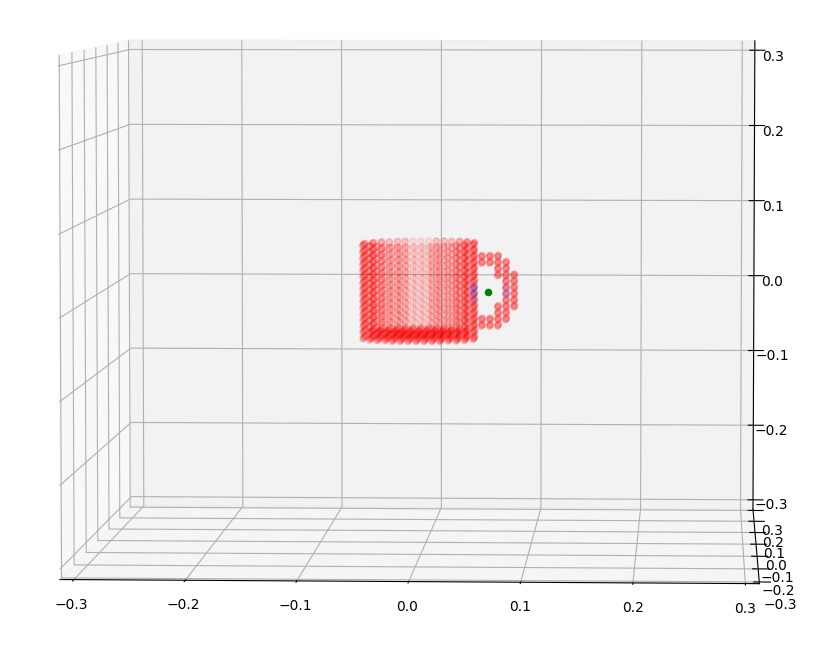
\includegraphics[width=\linewidth]{figures/virtual/3.png}
%         \caption{}
%     \end{subfigure}
%     \begin{subfigure}{(\linewidth - 0.1\linewidth)/6}
%         \centering
%         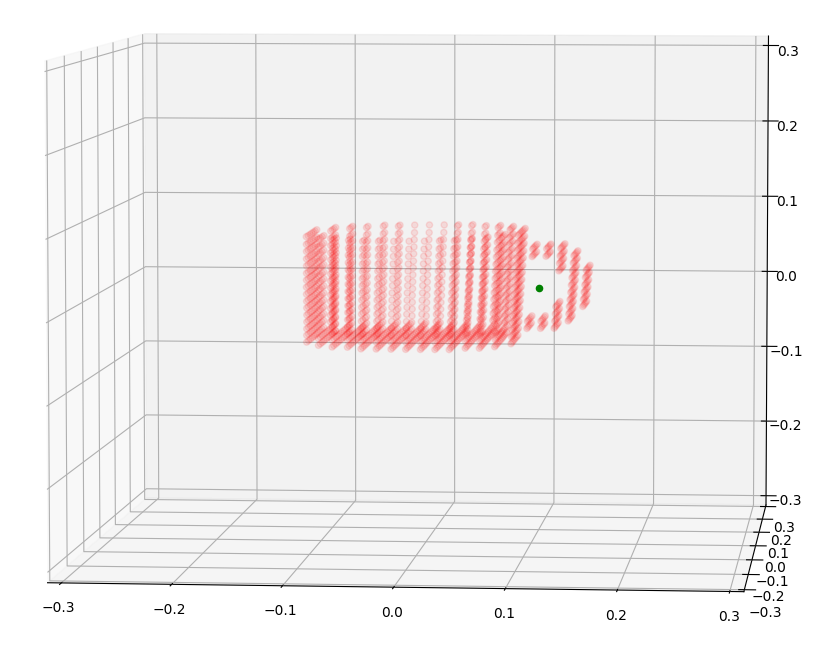
\includegraphics[width=\linewidth]{figures/virtual/4.png}
%         \caption{}
%     \end{subfigure}
%     \begin{subfigure}{(\linewidth - 0.1\linewidth)/6}
%         \centering
%         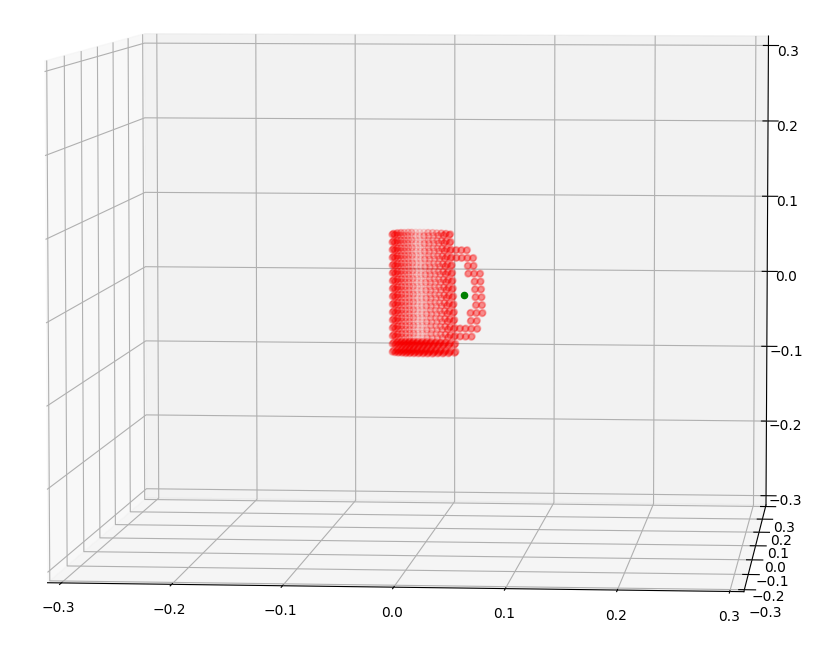
\includegraphics[width=\linewidth]{figures/virtual/5.png}
%         \caption{}
%     \end{subfigure}
%     \begin{subfigure}{(\linewidth - 0.1\linewidth)/6}
%         \centering
%         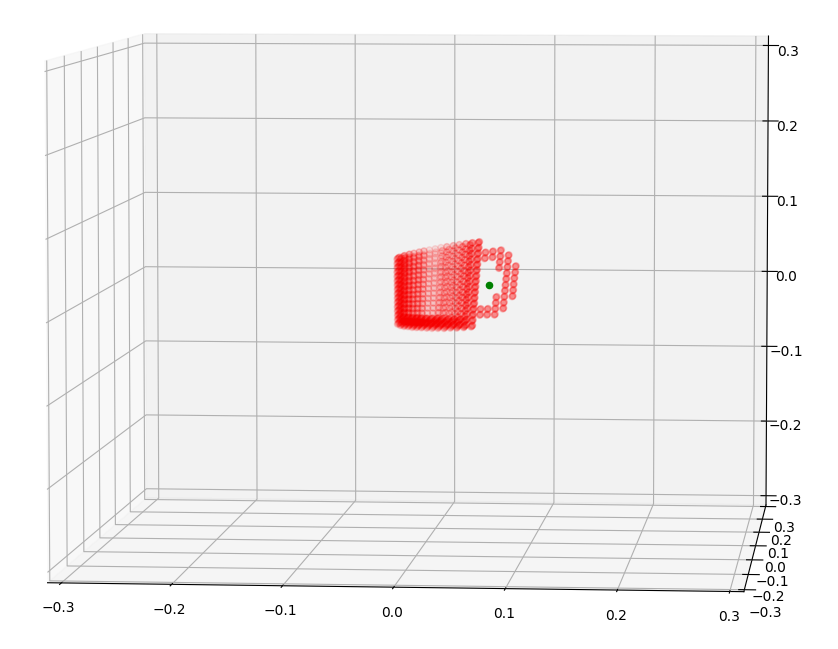
\includegraphics[width=\linewidth]{figures/virtual/6.png}
%         \caption{}
%     \end{subfigure}
%     \caption{Sketch: (a): a demonstration of the mug tree task, (b) a virtual point (green) in the middle of the mug's handle, (c) 10 (?) nearest neighbors (blue\ob{almost invisible, I know}), (d-f) warping the virtual point together with the mug.}
%     \label{fig:virtual_points}
% \end{figure*}

\section{Limitations}


\section{Conclusion}

Object decomposition / part segmentation \cite{tenorth13decomposing,vahrenkamp16partbased,chen22neural}

%===============================================================================

\clearpage

%===============================================================================

% no \bibliographystyle is required, since the corl style is automatically used.
\bibliography{main,zotero}  % .bib

\clearpage
\appendix

\section{Method Details}
\label{appendix:method}

\begin{algorithm}[H]

\caption{Warp Learning}\label{alg:warp_learn} 

\begin{flushleft}
    \hspace*{\algorithmicindent} \textbf{Input:} Meshes of $K$ example object instances $\{ \mathrm{obj}_1, \mathrm{obj}_2, ..., \mathrm{obj}_K \}$. \\
    \hspace*{\algorithmicindent} \textbf{Output:} Canonical point cloud, vertices and faces and a latent space of warps. \\
    \hspace*{\algorithmicindent} \textbf{Parameters:} Smoothness of CPD warping $\alpha$ and number of PCA components $L$.
\end{flushleft}

\begin{algorithmic}[1]

    \State $\mathrm{PCD} = \left< \mathrm{SampleS}(\mathrm{obj}_i) \right>_{i=1}^K$. \Comment{\textcolor{blue}{Sample a small point cloud per object (Appendix \ref{appendix:method:sampling}).}}
    \State $C = \mathrm{SelectCanonical}(\mathrm{PCD})$. \Comment{\textcolor{blue}{Select a canonical object with index $C$ (Appendix \ref{appendix:method:canonical}).}}
    \State $\mathrm{canon} = \mathrm{Concat}(\mathrm{obj}_C.\mathrm{vertices}, \mathrm{SampleL}(\mathrm{obj}_C))$. \Comment{\textcolor{blue}{Use both vertices and surface samples.}}
    \For {$i \in \{ 1, 2, ..., K \}, i \neq C$}
        \State $W_{C \rightarrow i} = \mathrm{CPD}(\mathrm{canon}, \mathrm{PCD}_i, \alpha)$. \Comment{\textcolor{blue}{Coherent Point Drift warping (Section \ref{sec:background}).}}
    \EndFor
    \State $D_W = \{ \mathrm{Flatten}(W_{C \rightarrow i}) \}_{i = 1, i \neq C}^K$. \Comment{\textcolor{blue}{Dataset of displacements of $\mathrm{canon}$.}}
    \State $\mathrm{PCA} = \mathrm{FitPCA}(D_W, \mathrm{n\_components}=L)$. \Comment{\textcolor{blue}{Learn a latent space of canonical object warps.}}
    \State \Return $\mathrm{Canon}(\mathrm{points} = \mathrm{canon}, \mathrm{vertices} = \mathrm{obj}_C.\mathrm{vertices}, \mathrm{faces} = \mathrm{obj}_C.\mathrm{faces}), \mathrm{PCA}$.

\end{algorithmic}

\end{algorithm}

\begin{algorithm}[H]

\caption{Warp Inference and Mesh Reconstruction}\label{alg:warp_infer} 

\begin{flushleft}
    \hspace*{\algorithmicindent} \textbf{Input:} Observed point cloud $\mathrm{pcd}$, canonical object $\mathrm{canon}$ and latent space $\mathrm{PCA}$. \\
    \hspace*{\algorithmicindent} \textbf{Output:} Predicted latent shape $v$ and pose $T$. \\
    \hspace*{\algorithmicindent} \textbf{Parameters:} Number of random starts $S$, number of gradient descent steps $T$, learning rate $\eta$ and object size regularization $\beta$.
\end{flushleft}

\begin{algorithmic}[1]

    \State $t_g = \frac{1}{|\mathrm{pcd}|} \sum_{i=1}^{|\mathrm{pcd}|} \mathrm{pcd}_i$.
    \State $\mathrm{pcd} = \mathrm{pcd} - t_g$. \Comment{\textcolor{blue}{Center the point cloud.}}
    \For {$i = 1$ \textbf{to} $S$}
        \State $R_{\mathrm{init}} =$ Random initial 3D rotation matrix.
        \State Initialize $v = \begin{pmatrix} 0 & 0 & ... & 0 \end{pmatrix}, s = \begin{pmatrix} 1 & 1 & 1 \end{pmatrix}, t_l = \begin{pmatrix} 0 & 0 & 0 \end{pmatrix}, \hat{R} = \begin{pmatrix} 1 & 0 & 0 \\ 0 & 1 & 0 \end{pmatrix}$.
        \State Initialize $\mathrm{Adam}$ \cite{kingma17adam} with parameters $v, s, t_l, r$ and learning rate $\eta$.
        \For {$j = 1$ \textbf{to} $T$}
            \State $\delta = \mathrm{Reshape}(Wv)$.
            \State $X = \mathrm{canon.points} + \delta$. \Comment{\textcolor{blue}{Warped canonical point cloud.}}
            \State $R = \mathrm{GramSchmidt(\hat{R})}$.
            \State $X = (X \odot s) R_{\mathrm{init}}^T R^T + t_l$. \Comment{\textcolor{blue}{Scaled, rotated and translated point cloud.}}
            \State $\mathcal{L} = \frac{1}{|\mathrm{pcd}|} \sum_k^{|\mathrm{pcd}|} \min_l^{|X|} \norm{\mathrm{pcd}_k - X_l}_2^2$. \Comment{\textcolor{blue}{One-sided Chamfer distance.}}
            \State $\mathcal{L} = \mathcal{L} + \beta \max_l^{|X|} \norm{X_l}_2^2$. \Comment{\textcolor{blue}{Object size regularization.}}
            \State Take a gradient descent step to minimize $\mathcal{L}$ using $\mathrm{Adam}$.
        \EndFor
    \EndFor
    \State Find parameters $v^*, s^*, t^*_l, R_{\mathrm{init}}^*, R^*$ with the lowest final loss across $i \in \{ 1, 2, ..., S \}$.
    \State $X = \mathrm{canon.points} +\mathrm{Reshape}(W v^*)$.
    \State $X = (X \odot s^*) (R_{\mathrm{init}}^*)^T (R^*)^T + t^*_l + t_g$. \Comment{\textcolor{blue}{Complete point cloud in workspace coordinates.}}
    \State $\mathrm{vertices} = \langle X_1, X_2, ..., X_{|\mathrm{canon.vertices}|} \rangle$. \Comment{\textcolor{blue}{First $|\mathrm{canon.vertices}|$ points of $X$ are vertices.}}
    \State \Return $\mathrm{Mesh}(\mathrm{vertices} = \mathrm{vertices}, \mathrm{faces} = \mathrm{canon.faces})$. \Comment{\textcolor{blue}{Warped mesh.}}

\end{algorithmic}

\end{algorithm} %\evdp{There is a lot of information here, is it possible to present the main steps here and leave the details for the appendix?}

\subsection{Point Cloud Sampling}
\label{appendix:method:sampling}

\subsection{Canonical Object Selection}
\label{appendix:method:canonical}

Among the $K$ example objects, we would like to find the one that is the easiest to warp to the other objects. For example, if we have ten examples of mugs, but only one mug has a square handle, we should not choose it as it might be difficult to warp it to conform to the round handles of the other nine mugs.

\begin{algorithm}[H]

\caption{Exhaustive Canonical Object Selection}\label{alg:canon_select_1} 

\begin{flushleft}
    \hspace*{\algorithmicindent} \textbf{Input:} Meshes of $K$ example object instances $\{ \mathrm{obj}_1, \mathrm{obj}_2, ..., \mathrm{obj}_K \}$. \\
    \hspace*{\algorithmicindent} \textbf{Output:} Canonical object $\mathrm{obj}^C$, $\mathrm{PCA}$ mapping latent vectors to warps of $\mathrm{obj}^C$. \\
\end{flushleft}

\begin{algorithmic}[1]

    \State x.

\end{algorithmic}

\end{algorithm}

\begin{algorithm}[H]

\caption{Approximate Canonical Object Selection}\label{alg:canon_select_2} 

\begin{flushleft}
    \hspace*{\algorithmicindent} \textbf{Input:} Meshes of $K$ example object instances $\{ \mathrm{obj}_1, \mathrm{obj}_2, ..., \mathrm{obj}_K \}$. \\
    \hspace*{\algorithmicindent} \textbf{Output:} Canonical object $\mathrm{obj}^C$, $\mathrm{PCA}$ mapping latent vectors to warps of $\mathrm{obj}^C$. \\
\end{flushleft}

\begin{algorithmic}[1]

    \State x.

\end{algorithmic}

\end{algorithm}

\section{Experiment Details}
\label{appendix:experiment}

\subsection{Object re-arrangement on a physical robot}
\label{appendix:experiment:rearrangement}

\end{document}
